\documentclass[10pt]{beamer}
%\documentclass[handout,10pt]{beamer}
\usepackage{my_style}

%%%%%%%%%%%%%%%%%%%%%%%%%%%%%%%%%%%%%%%%%%%%%%%%%%%%%%%%%%%%%
%%%%%%%%%%%%%%%%%%%%%%%%%%%%%%%%%%%%%%%%%%%%%%%%%%%%%%%%%%%%%

\title[Math/CS 375]{Lecture 03 - A}
\subtitle{\S 4.3 Numerical Differentiation}

\begin{document}
% -------------------------------------------------
\begin{frame}
  \titlepage
\end{frame}
% -------------------------------------------------

\begin{frame}{Goals}
We will answer these questions:\\[3mm]
\begin{itemize}
    \item What is the Taylor expansion of $f(x\pm h)$?
    \item How is the Taylor expansion used to develop finite difference schemes?
    \item How can we compare the performance of various finite difference algorithms?
    \item What is the central difference scheme and what makes it different from the forward or backward difference schemes? 
\end{itemize}
\end{frame}

\begin{frame}
\frametitle{Problem Statement}
\begin{block}{Given}
  \begin{itemize}
      \item Some function $y=f(x)$
      \item A point $x_0$
      \item You may evaluate $f$ at discrete locations e.g. $f(x_0+h)$, $f(x_0)$ and $f(x_0-h)$
  \end{itemize}
\end{block}

\begin{block}{Objective}
  \begin{itemize}
      \item Approximate numerical value of $f'(x_0)$
  \end{itemize}
\end{block}

\vspace{4mm}
\begin{center}
Think of $f(x)$ as a black box. You cannot visualize $f$ but you can input numbers and get an output. 
\end{center}

\end{frame}
%%%%%%%%%%%%%%%%%%%%%%%%%%%%%%%%%%%%%%%%%%%%%%%%%%%%
\sectionframe{Taylor Series}
%%%%%%%%%%%%%%%%%%%%%%%%%%%%%%%%%%%%%%%%%%%%%%%%%%%%

\begin{frame}[shrink]{Taylor Expansion}

\begin{itemize}
    \item Recall the Taylor series expansion of $f(x)$ around $x_0$
    $$
        f(x) =  f(x_0) + (x-x_0) f'(x_0) + \frac{(x-x_0)^2}{2!} f''(x_0) + \dots + \frac{(x-x_0)^n}{n!} f^{(n)}(x_0)+\dots
    $$
    \item Let $x = x_0 + h$
    \begin{align*}    
    f(x_0 + h) &= f(x_0) + (x_0 + h -x_0) f'(x_0) + \\
                 &\frac{(x_0 + h -x_0)^2}{2!} f''(x_0) + \dots + \frac{(x_0 + h -x_0)^n}{n!} f^{(n)}(x_0)+\dots
    \end{align*}


    \begin{block}{Alternate Taylor Expansion Formula}
    $$
        f(x_0 + h) =  f(x_0) + h f'(x_0) + \frac{h^2}{2!} f''(x_0) + \dots + \frac{h^n}{n!} f^{(n)}(x_0)+\dots
    $$
    \end{block}
    \begin{block}{Expansion with $-h$}
    $$
        f(x_0 - h) =  f(x_0) - h f'(x_0) +\frac{h^2}{2!} f''(x_0) + \dots + (-1)^n\frac{h^n}{n!} f^{(n)}(x_0)+\dots
    $$
    \end{block}
\end{itemize}
\end{frame}
%%%%%%%%%%%%%%%%%%%%%%%%%%%%%%%%%%%%%%%%%%%

\begin{frame}{Compare Taylor Expansion Formulas}


\begin{block}{
Regular Taylor Series
}
    $$
        f(x) =  f(x_0) + (x-x_0) f'(x_0) + \frac{(x-x_0)^2}{2!} f''(x_0) + \dots + \frac{(x-x_0)^n}{n!} f^{(n)}(x_0)+\dots
    $$
\begin{itemize}
    \item Interested in approximating $f(x)$ 
    \item Approximation centered around $x_0$
\end{itemize}
\end{block}

\begin{center}
    v.s.
\end{center}

\begin{block}{ Alternate Taylor Series }
    $$
        f(x_0 + h) =  f(x_0) + h f'(x_0) + \frac{h^2}{2!} f''(x_0) + \dots + \frac{h^n}{n!} f^{(n)}(x_0)+\dots
    $$
    \begin{itemize}
    \item Interested in a small perturbation away from $f(x_0)$ 
    \item Approximation centered around $x_0$
\end{itemize}
\end{block}

\end{frame}
%%%%%%%%%%%%%%%%%%%%%%%%%%%%%%%%%%%%%%%%%%%
\begin{frame}{Strategy}
\begin{itemize}
    \item Use Taylor Series
    \begin{align*}
        f(x+h) &= f(x) + h f'(x) + \frac{h^2}{2}f''(\xi),\;\;\;\;\;\;\;\;\; \mbox{ for } \xi \in [x, x+h]\\
        f(x-h) &= f(x) - h f'(x) + \frac{h^2}{2}f''(\xi),\;\;\;\;\;\;\;\;\; \mbox{ for } \xi \in [x-h, x]
    \end{align*}
    \item Don't worry about $\xi$, some unknown point in the interval
    \item Manipulate, add, and then subtract the above Taylor Series to obtain a formula for $f'(x)$
\end{itemize}
\end{frame}
%%%%%%%%%%%%%%%%%%%%%%%%%%%%%%%%%%%%%%%%%%%
\sectionframe{Forward Difference}
%%%%%%%%%%%%%%%%%%%%%%%%%%%%%%%%%%%%%%%%%%%

\begin{frame}{First attempt: Taylor}

Let's find an approximate formula for $f'(x)$\\[4mm]

\begin{itemize}
    \item Taylor series:
    \begin{equation*}
      f(x+h) = f(x) + h f'(x) + \frac{h^2}{2}f''(\xi)
    \end{equation*}
    \item Slight rearrangement
    \begin{equation*}
      f'(x) = \frac{f(x+h)-f(x)}{h} - \xxcancel{\frac{h}{2}f''(\xi)}
    \end{equation*}
    \item<2-> If we ignore the last term, we have our approximation 
        $$
        f'(x) \approx \frac{f(x+h)-f(x)}{h}
        $$
\end{itemize}
\end{frame}

%%%%%%%%%%%%%%%%%%%%%%%%%%%%%%%%%%%%%%%%%%%
\begin{frame}{Approximation and Error}

    \begin{equation*}
      \underbrace{f'(x)}_{\textrm{true value}} = \underbrace{\frac{f(x+h)-f(x)}{h}}_{\textrm{approximation}} - \underbrace{\frac{h}{2}f''(\xi)}_{igonre}
    \end{equation*}
    
    \begin{itemize}
        \item We have a method to approximate the derivative 
        \item Notice that we have a \textit{formula for the error}
        \item Absolute error 
        \begin{align*}
        E &= |\text{true} - \text{approx}|\\
           &= \left|f'(x) - \tfrac{f(x+h)-f(x)}{h} \right|\\
           &= \left|-\frac{h}{2}f''(\xi) \right|\\
        \end{align*}
    \end{itemize}
\end{frame}
%%%%%%%%%%%%%%%%%%%%%%%%%%%%%%%%%%%%%%%%%%%
\begin{frame}{Forward Difference}

Approximation
\begin{equation*}
  f'(x) \approx \frac{f(x+h)-f(x)}{h}
\end{equation*}
with an absolute error of
\begin{equation*}
  E=\frac{h}{2}|f''(\xi)| 
\end{equation*}

\method{Forward Difference}{function $f(x)$, step parameter $h$}{approximation to $f'(x)$}{Obtain a parameterized value for $f'(x_0)$ mechanically.}

\end{frame}

%%%%%%%%%%%%%%%%%%%%%%%%%%%%%%%%%%%%%%%%%%%
\sectionframe{Evaluating Performance}
%%%%%%%%%%%%%%%%%%%%%%%%%%%%%%%%%%%%%%%%%%%

\begin{frame}{Evaluating Performance}

\begin{block}{Algorithm}
\begin{itemize}
    \item Goal: approximate $f'(x_0)$
    \item Given: $f(x)$, $h$, and $x_0$
    \item Method: $f'(x) \approx \dfrac{f(x_0+h)-f(x_0)}{h}$
\end{itemize}
\end{block}

\question{
\begin{itemize}
    \item What happens if we decrease $h$? 
    \item Does the error decrease slowly?
    \item Does the error decrease quickly?
    \item How do you quantify such a thing?\
    \item<2> \textbf{How do we describe the algorithm's perform?}
\end{itemize}
} 
\end{frame}

%%%%%%%%%%%%%%%

\begin{frame}{Convergence Rate}

\begin{center}
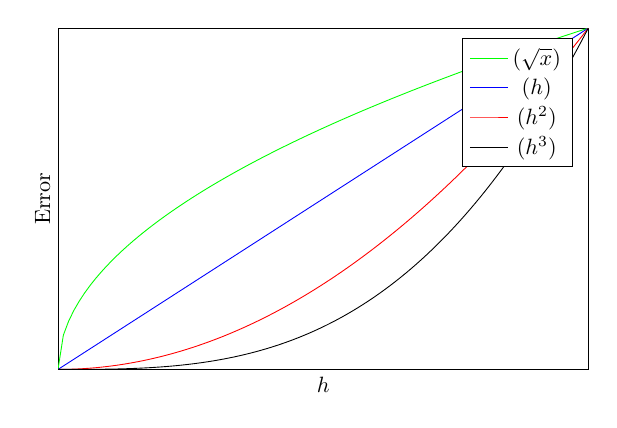
\begin{tikzpicture}[scale=0.8]
\begin{axis}[
    xlabel={$h$},
    ylabel={Error},
    xmin=0, xmax=1,
    ymin=0, ymax=1,
    legend pos=north east,
    grid=both,
    major grid style={line width=.2pt,draw=gray!50},
    width=10cm,
    height=7cm,
    xtick=\empty,
    ytick=\empty]
\addplot[green,domain=0:1,samples=100] {sqrt(x)};
\addlegendentry{$\mO(\sqrt{x})$}
\addplot[blue,domain=0:1,samples=100] {x};
\addlegendentry{$\mO(h)$}
\addplot[red,domain=0:1,samples=100] {x^2};
\addlegendentry{$\mO(h^2)$}
\addplot[black,domain=0:1,samples=100] {x^3};
\addlegendentry{$\mO(h^3)$}
\end{axis}
\end{tikzpicture}
\end{center}

\begin{itemize}
    \item We know error decreases with respect  $h\rightarrow 0$. 
    \item For the time being let's assume that error is algebraic 
    $$E = \mO(h^p)$$
    \item Bigger $p$ $\implies$ better algorithm
\end{itemize}
\end{frame}

%%%%%%%%%%%%%%%%%%%%%%%%%%%%%%%%%%%%%%%%%%%
\begin{frame}{Testing Order of Convergence}

\begin{block}{Assumption}
    Assume error decreases like $E= \mO(h^p)$.
\end{block}


    \vspace{3mm}
\begin{block}{Numerical Experiment}
    \begin{enumerate}
        \item Implement your algorithm as a function of $h$
        \item Choose a test function $y=f(x)$ whose true derivative $f'(x)$ is known
        \item Choose two values for $h$ e.g. $h_1 = 0.01$, $h_2 = 0.00001$
        \item For each $h$, use your code to approximate $f'(x)$ and compute the error
        \item Calculate 
            \begin{equation*}
                p = \frac{ \log(E_1/E_2) }{ \log(h_1/h_2) }
            \end{equation*}
    \end{enumerate}
\end{block}
\end{frame}
%%%%%%%%%%%%%%%%%%%%%%%%%%%%%%%%%%%%%%%%%%%
\begin{frame}{Derivation}
    Let $E=\mO(h^p)$. 
    \vspace{3mm}
    \begin{itemize}
        \item Calculate the error for two different values of $h$
            $$E_1 \approx c h_1^p \quad\quad E_2 \approx c h_2 ^p $$
        \item Compute ratio 
            $$\frac{E_1}{E_2} \approx \frac{c h_1^p}{c h_2 ^p} = \left(\frac{h_1}{h_2}\right)^p$$
        \item Take the log 
            $$ \log\left(\frac{E_1}{E_2}\right) \approx  p \log\left(\frac{h_1}{h_2}\right)$$
        \item Thus  
            $$p = \frac{ \log(E_1/E_2) }{ \log(h_1/h_2) }$$
    \end{itemize}
\end{frame}

%%%%%%%%%%%%%%%%%%%%%%%%%%%%%%%%%%%%%%%%%%%
\begin{frame}{Numerical Test  \texttt{diff\_fwd.m} }
\vspace{-5pt}

\begin{itemize}
    \item Consider
    \begin{equation*}
      f(x) = \sin(\pi x)\,\, \text{on}\,\, [-1,1]
    \end{equation*}
    \item Approximate $f'(x) = \pi \cos(\pi x)$ with
    \begin{equation*}
      f'(x) \approx \frac{f(x+h)-f(x)}{h}
    \end{equation*}
    \item Compute
    \begin{equation*}
      p = \frac{ \log(\text{err}_k/\text{err}_j) }{ \log(h_k/h_j) }
    \end{equation*}

    \item Results: 
\end{itemize}
    \vspace{3mm}

    \begin{center}
        See \texttt{diff\_fwd.m}
    \end{center}
\end{frame}

%%%%%%%%%%%%%%%%%%%%%%%%%%%%%%%%%%%%%%%%%%%
\begin{frame}{Plotting Convergence}

    \textbf{How to display experimental rate of convergence}:
    \begin{enumerate}
        \item Implement your algorithm as a function of $h$
        \item Choose a test function $y=f(x)$ whose true derivative $f'(x)$ is known
        \item Choose a range of values for $h$ e.g. $h = 1/2, 1/4, 1/8, 1/16, \ldots$
        \item For each $h$, use your code to approximate $f'(x)$ and compute the error
        \item Tabulate the results

    \begin{table}[]
        \centering
        \begin{tabular}{c|c|c|c|c}
            $h$ & 1/2 & 1/4 & 1/8 & 1/16\\\hline
            Error &   &     &     & 
        \end{tabular}
        \label{tab:my_label}
    \end{table}
        \item Plot Error versus $h$ on a log-log plot or a log-linear plot
    \end{enumerate}

        \vspace{3mm}

    \begin{center}
        See \texttt{diff\_fwd\_plot.m}
    \end{center}
\end{frame}
%%%%%%%%%%%%%%%%%%%%%%%%%%%%%%%%%%%%%%%%%%%
\begin{frame}{Plotting Convergence}
    \begin{figure}
        \centering
        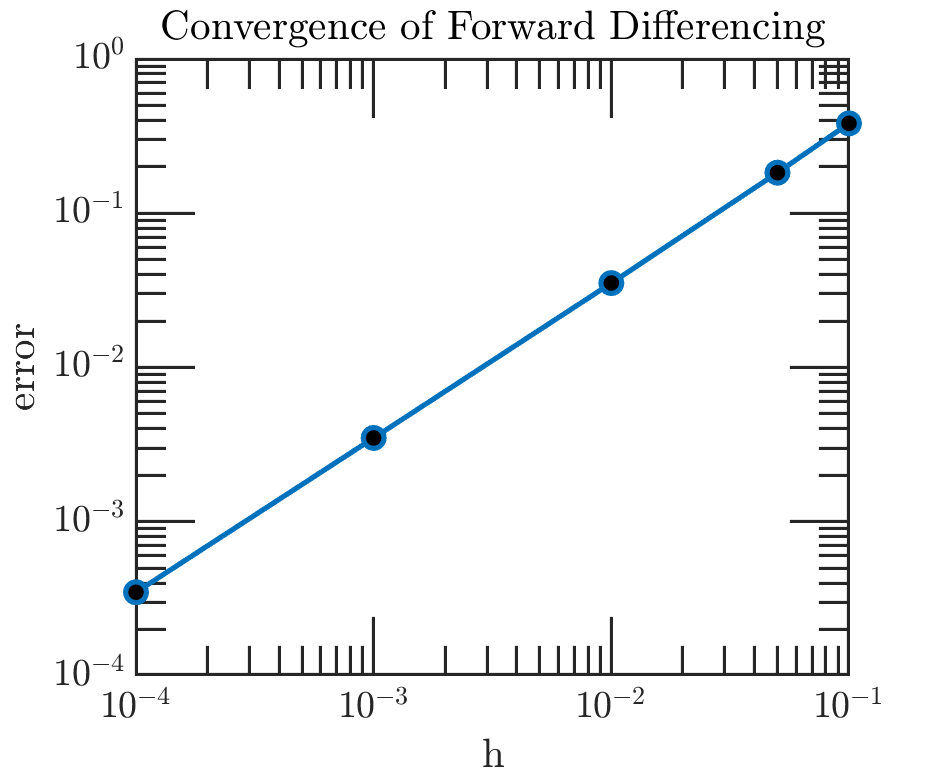
\includegraphics[width=0.6\linewidth]{figs/fd_convergence.png}
        % \caption{Caption}
        % \label{fig:enter-label}
    \end{figure}
    \begin{itemize}
        \item This is a log-log plot 
        \item $h$ decreases going from right to left
        \item As $h$ decreases, the error decreases 
    \end{itemize}
\end{frame}

%%%%%%%%%%%%%%%%%%%%%%%%%%%%%%%%%%%%%%%%%%%
\begin{frame}{Assessing Convergence Rate}
    \begin{figure}
        \centering
        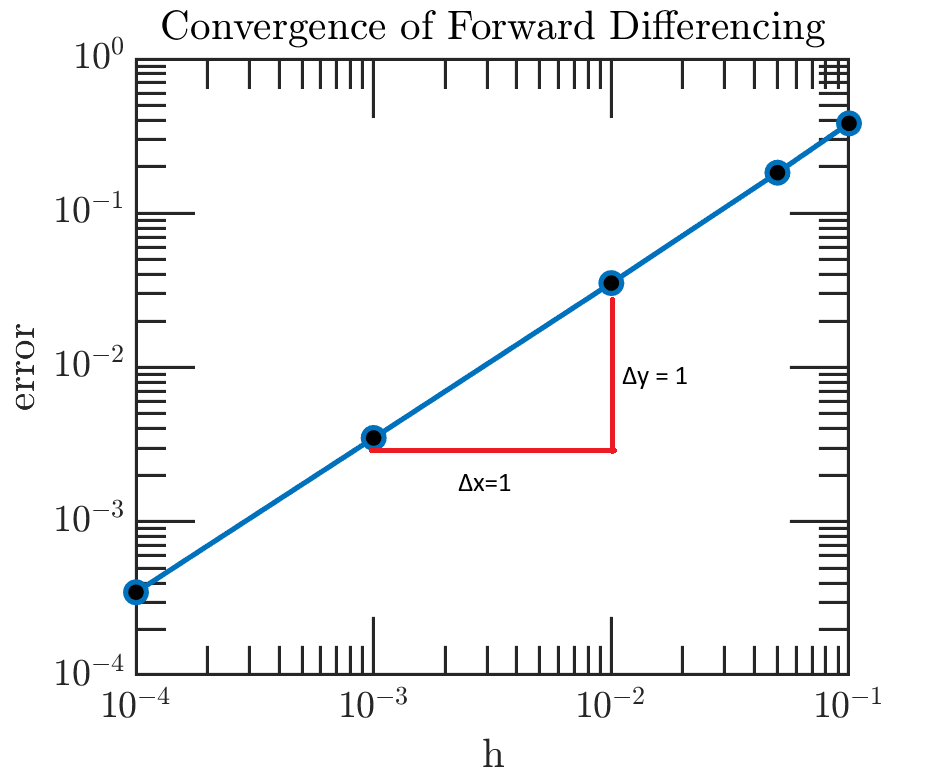
\includegraphics[width=0.5\linewidth]{figs/fd_convergence_edit.png}
        % \caption{Caption}
        % \label{fig:enter-label}
    \end{figure}
    \begin{itemize}
        \item If $E=Ch^p$, then $\log(E) = p\log(h)+K$ so the slope must be $p$
    \end{itemize}
    \keyidea{Count the slope on the log-log plot to find $p$. Forward difference plot shows $p=1$.}
\end{frame}

%%%%%%%%%%%%%%%%%%%%%%%%%%%%%%%%%%%

\begin{frame}{Performance Metric}
\begin{itemize}
    \item Experimentally, we have found that the forward difference has an error
    $$
    E = \mO(h^P), \quad p=1
    $$
    \define{Order of Accuracy}{
    The integer $p$ in $E=\mO(h^p)$ is called the \textbf{order of accuracy}. 
    }

    \item We say that forward difference scheme is 
    $$
    \text{"first-order accurate"}
    $$

\end{itemize}
\end{frame}
%%%%%%%%%%%%%%%%%%%%%%%%%%%%%%%%%%%%%%%%%%%
\begin{frame}{Truncation Error}

\begin{itemize}
    \item The term ignored in the Taylor expansion \textit{is} the error term

    \begin{equation*}
      \underbrace{f'(x)}_{\textrm{true value}} = \underbrace{\frac{f(x+h)-f(x)}{h}}_{\textrm{approximation}} - \underbrace{\frac{h}{2}f''(\xi)}_{igonre}
    \end{equation*}
    
    \vfill
    
    \item The error depends on $f''$, $\xi$ and $h$
        but $f''(\xi)$ is roughly constant if $f$ is smooth so we write
        $$error =\frac{h}{2} \left|f''(\xi)\right|\approx Ch=\mO(h)$$
        \vfill
        
    \keyidea{
    The theoretical error terms is called the truncation error. The truncation error tells use the order of accuracy.
    }
\end{itemize}
\end{frame}

%%%%%%%%%%%%%%%%%%%%%%%%%%%%%%%%%%%%%%%%%%%
\sectionframe{Backward Difference}
%%%%%%%%%%%%%%%%%%%%%%%%%%%%%%%%%%%%%%%%%%%
\begin{frame}{Backward Difference}
    \begin{itemize}
        \item Let's derive another differentiation scheme with the backward Taylor expansion
\begin{align*}
f(x-h) &= f(x) - h f'(x) + \frac{h^2}{2}f''(\xi)\\
\onslide<2->{f(x-h)-f(x) &=  - h f'(x) + \frac{h^2}{2}f''(\xi)}\\
\onslide<3->{\frac{f(x-h)-f(x)}{h} &=  -  f'(x) + \frac{h}{2}f''(\xi)}\\
\onslide<4->{\frac{f(x)-f(x-h)}{h} &=  f'(x) - \frac{h}{2}f''(\xi)}\\
\end{align*}
    \item<5> We have a new scheme 
    $$
    \underbrace{\frac{f(x)-f(x-h)}{h}}_{approx} =  \underbrace{f'(x)}_{true} - \underbrace{\frac{h}{2}f''(\xi)}_{ignore}
    $$
    \end{itemize}
\end{frame}
%%%%%%%%%%%%%%%%%%%%%%%%%%%%%%%%%%%%%%%%%%%
\begin{frame}{Backward Difference}
\begin{itemize}
    \item This approximation is called the \textbf{backward difference scheme}
\begin{equation*}
  f'(x) \approx \frac{f(x)-f(x-h)}{h}
\end{equation*}
    \item Error is also first-order accurate
\end{itemize}
\begin{equation*}
  \text{error} = \frac{h}{2}f''(\xi) = \mathcal{O}(h)
\end{equation*}

\method{Backward Difference}
{function $f(x)$, step parameter $h$}
{approximation to $f'(x)$}
{Similar to forward difference but it looks at a prior point}

\end{frame}

%%%%%%%%%%%%%%%%%%%%%%%%%%%%%%%%%%%%%%%%%%%
\sectionframe{Central Difference}
%%%%%%%%%%%%%%%%%%%%%%%%%%%%%%%%%%%%%%%%%%%
\begin{frame}{Can we do better?}
\begin{itemize}
    \item Look at the Forward AND Backward Taylor series together
    \begin{align*}
      f(x+h) & = f(x) + h f'(x) + \frac{h^2}{2}f''(x) + \frac{h^3}{6}f'''(x) + \frac{h^4}{24}f''''(\xi_{+})\\
      f(x-h) & = f(x) - h f'(x) + \frac{h^2}{2}f''(x) - \frac{h^3}{6}f'''(x) + \frac{h^4}{24}f''''(\xi_{-})\\
    \end{align*}

    \item<2-> Subtract them:
    \begin{equation*}
      f(x+h) - f(x-h) = 2 h f'(x) + \frac{h^3}{3}f'''(x) + \mathcal{O}(h^4)
    \end{equation*}
    \item<3-> Thus
    \begin{equation*}
      f'(x) = \frac{f(x+h) - f(x-h)}{2 h} - \frac{h^2}{6}f'''(x) + \mathcal{O}(h^3)
    \end{equation*}
\end{itemize}
\end{frame}
%%%%%%%%%%%%%%%%%%%%%%%%%%%%%%%%%%%%%%%%%%%
\begin{frame}{Truncation Error}
    \begin{itemize}
        \item Subtracting $f(x+h)$ and $f(x-h)$ cancels out even powers and odd powers 
            \begin{align*}
      f(x+h) & = f(x) + h f'(x) + \frac{h^2}{2}f''(x) + \frac{h^3}{6}f'''(x) + \frac{h^4}{24}f''''(\xi_{+})\\
      f(x-h) & = f(x) - h f'(x) + \frac{h^2}{2}f''(x) - \frac{h^3}{6}f'''(x) + \frac{h^4}{24}f''''(\xi_{-})\\
    \end{align*}

    \item The truncation error (true - approx) has the form 
    \begin{align*}
         f'(x) - \frac{f(x+h) - f(x-h)}{2 h} &= - \frac{h^2}{3!}f'''(x) - \frac{h^4}{5!}f^{(5)}(x) - \frac{h^6}{7!}f^{(7)}(x) - \cdots\\
          &= c_2 h^2 + c_4 h^4 + \ldots
    \end{align*}

    \end{itemize}
    
\end{frame}
%%%%%%%%%%%%%%%%%%%%%%%%%%%%%%%%%%%%%%%%%%%
\begin{frame}{Central Difference - The Method}
Approximation
\begin{equation*}
  f'(x) = \frac{f(x+h) - f(x-h)}{2 h} + \frac{h^2}{6}f'''(x) + \mathcal{O}(h^3)
\end{equation*}
with truncation error of
\begin{equation*}
  \text{error} = - \frac{h^2}{6}f'''(\xi) = \mathcal{O}(h^2)
\end{equation*}

\bigskip
\method{Central Difference}
{function $f(x)$, step parameter $h$}
{approximation to $f'(x)$}
{improvement over the forward and backward difference methods}

\end{frame}
%%%%%%%%%%%%%%%%%%%%%%%%%%%%%%%%%%%%%%%%%%%
\begin{frame}{What's with the Names?}
\begin{itemize}
    \item Forward difference looks forward
          \[f'(x) \approx \frac{f(x+h) - f(x)}{h}\]
          \vspace{-18pt}
          \begin{center}
          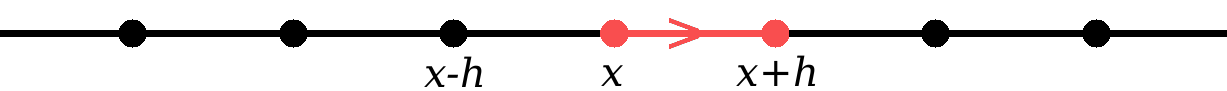
\includegraphics[scale=0.23]{./figs/forwarddiff.png}
          \end{center} \smallskip
    \item<2-> Backward difference looks backward
          \[f'(x) \approx \frac{f(x) - f(x-h)}{h}\]
          \vspace{-18pt}
          \begin{center}
          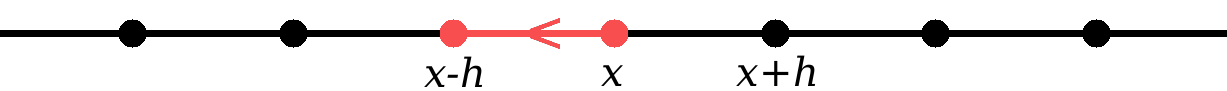
\includegraphics[scale=0.23]{./figs/backwarddiff.png}
          \end{center} \smallskip
    \item<3-> Central difference centers the subtraction around $x$
          \[f'(x) \approx \frac{f(x+h) - f(x-h)}{2 h}\]
          \vspace{-18pt}
          \begin{center}
          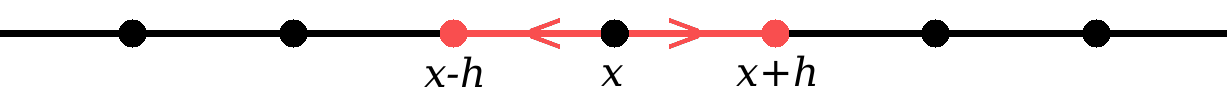
\includegraphics[scale=0.23]{./figs/centraldiff.png}
          \end{center}
\end{itemize}
\end{frame}

%%%%%%%%%%%%%%%%%%%%%%%%%%%%%%%%%%%%%%%%%%%
\begin{frame}{Performance?}
\begin{itemize}
    \item In theory, the error for forward difference is 
     $$ E_{fwd} = \frac{h}{2}|f''(\xi)|$$
    \item Error for central difference is 
     $$ E_{cen} = \frac{h^2}{6} |f'''(\xi)|$$
\end{itemize}
    \question{
    \begin{itemize}
        \item What does this mean about the two algorithms?
        \item Which one is better?
    \end{itemize}
        }
\end{frame}
%%%%%%%%%%%%%%%%%%%%%%%%%%%%%%%%%%%%%%%%%%%
\begin{frame}{Numerical Test, \texttt{diff\_central.m}}
Same test as before 
\begin{itemize}
    \item Consider
    \begin{equation*}
      f(x) = \sin(\pi x)\,\, \text{on}\,\, [-1,1]
    \end{equation*}
    \item Use centered difference
    \begin{equation*}
      f'(x) \approx \frac{f(x+h)-f(x-h)}{2 h}
    \end{equation*}
    \item Calculate
    \begin{equation*}
      p = \frac{ \log(\text{err}_k/\text{err}_j) }{ \log(h_k/h_j) }
    \end{equation*}
    \item We are expecting $p\approx 2$
\end{itemize}
\vspace{4mm}
    \begin{center}
        See \texttt{diff\_central.m}
    \end{center} 
\end{frame}

%%%%%%%%%%%%%%%%%%%%%%%%%%%%%%%%%%%%%%%%%%%
\begin{frame}{Comparison in Convergence}

\begin{figure}
    \centering
    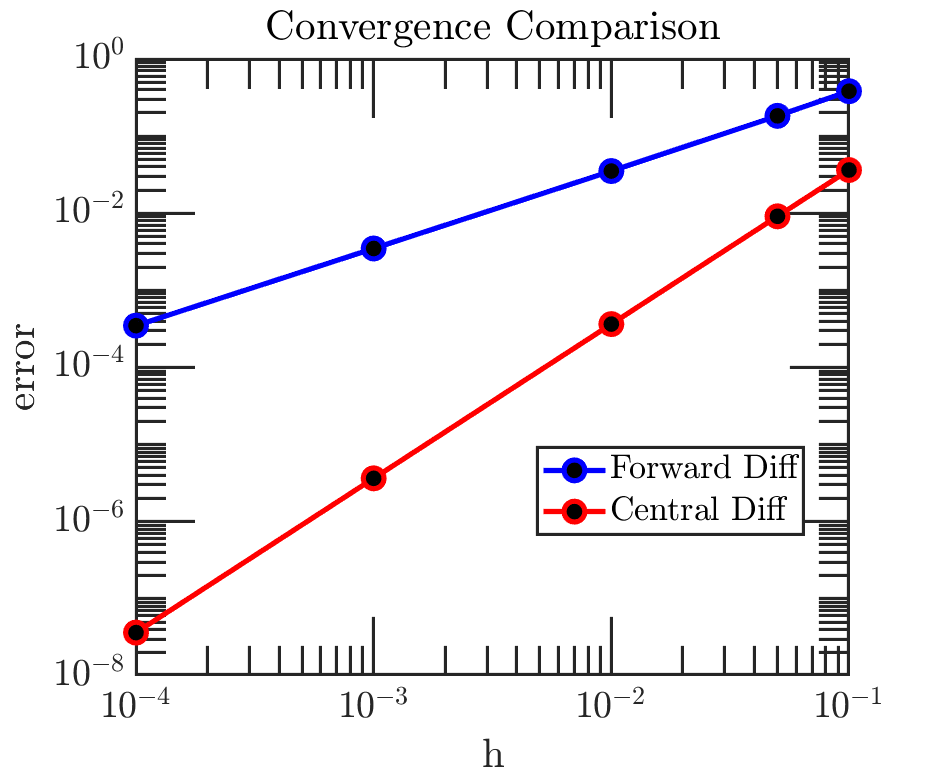
\includegraphics[width=0.6\linewidth]{figs/fd_cd_comparison.png}
\end{figure}

\keyidea{Since central difference is 2nd-order accurate, its error plummets to much faster as $h\to0^+$.}
\end{frame}
%%%%%%%%%%%%%%%%%%%%

\begin{frame}{Moving Forward}
\begin{itemize}
    \item Are there schemes that go beyond $\mO(h^2)$? 
\vfill
    \item Can we approximate higher order derivatives $f''(x)$?
\vfill

    \item How should the parameter $h$ be chosen in practice?
\vfill
\end{itemize}
    
\end{frame}

\end{document}
